\section{Case Studies}
\label{sec:caseStudy}
In order to quantify the effects of optimizing the scripts, we performed a case study.
We say that a C\# method is {\em intrinsicable} if it is a .NET Framework method for which the SCOPE compiler has a semantically equivalent C++ function.
The jobs were chosen based on a static analysis that found {\em optimizable vertices}.
An optimizable vertex is one that is implemented in C\#, but the C\# code calls only intrinsicable methods or user-defined functions, {\em UDFs}, where the UDF, in turn, calls only intrinsicable methods, and does not call any other UDFs, i.e., our inlining depth is one.
We then manually looked at the top jobs from  a ranked list (by CPU time) of jobs containing an optimizable vertex.

Because the input data for each job is not available, we needed to contact the job owners and ask them to re-run the job with a manually-inlined version of their script.
We were able to have \casestudyjobs{} jobs re-run by their owners.
We roughly categorize the jobs by their total CPU time: short, medium, and long.

\subsection{Optimizations With Effects On Job Algebra}
As explained in Section~\ref{sec:intro}, the optimizer may choose to modify the job algebra given the new information available to it.
For example, predicates might be pushed deeper into the DAG which can result in dramatic data reduction.
However, none of the case studies ended up causing this kind of optimization.


\subsection{Optimizations Without Effects On Job Algebra}
Even if the physical plan does not change, the resulting program might be might more efficient if it avoids the native to managed transition.
For SCOPE, the set of intrinsics means that by lifting more non-relational code into the parts of the program where such things are visible to the optimizer, more code can be executed in C++ instead of in C\#.

\begin{figure*}[ht]
\begin{tabular}{c|c|c|c|c|c} 
\toprule
  {\em Job Name} & {\em C++ translation}&{\em Job Cost} & \multicolumn{2}{c}{\em CPU time} &  {\em Throughput } \\
  \cmidrule{4-5}  
  & & & {\em Vertex Change} & {\em Job Change} &  \\
  \midrule

A & yes & medium & 59.63\%  & 23.00\% & 30\% \\
B &yes & medium & no change & no change & no change\\
C & yes & low    & 41.98\%  & 25.00\% & 38\% \\
D & no & - & - & - & -\\
E & yes & high   & 7.22\%   & 4.79\% &  5\% \\
F & yes & low & no change & no change & 115\% \\

%For Jobs A and B the numbers are averages over the a one week period.
\end{tabular}
\caption{Summary of case studies. The reported changes are percent improvements in CPU time and throughput. \label{fig:caseStudySummary}}
\end{figure*}

In total, we looked at \casestudyjobs{} re-run jobs, summarized in Figure~\ref{fig:caseStudySummary}. 
For one job (D), the optimization did not trigger C++ translation of an inlined operator because the operator called to a non-intrinsicable method that we mistakenly thought was an intrinsic.
After fixing this problem, we used the correct set of intrinsics to obtain data presented in Section~\ref{sec:evaluation}.
\begin{figure}[ht]
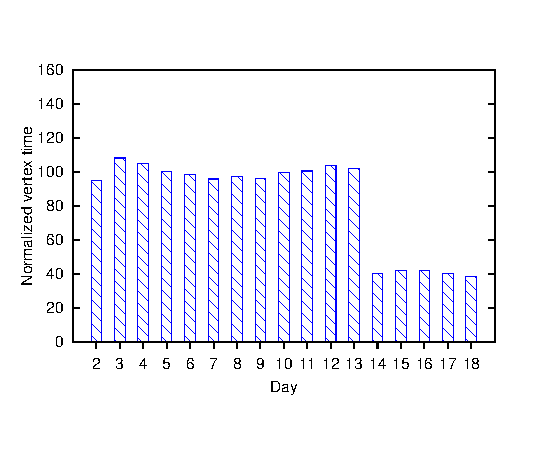
\includegraphics{graphs/normalizedTimesA}
\caption{Case Study A \label{fig:CaseStudyA}}
\end{figure}

\begin{figure}[ht]
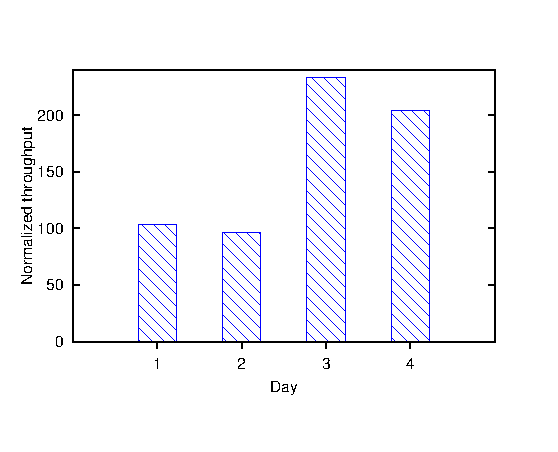
\includegraphics{graphs/throughtputF}
\caption{Case Study F \label{fig:CaseStudyF}}
\end{figure}


For jobs A and B, we were able to perfom the historical study over a period of 18 days. 
Both jobs are medium-expensive jobs, run daily and contain exactly one optimizable vertex due to a UDF. In both cases, inlining that UDF resulted in the entire vertex being executed in C++.
Figure~\ref{fig:CaseStudyA} shows the improvements in CPU time and throughput for an optimized vertex in Job A over an 18 day period, the last 5 of which were with the inlined UDF.
The values are normalized by the average of the unoptimized execution times; the optimized version saves approximately 60\% of the execution time.
However, the normalized vertex CPU time in Job B does not show any consistent improvement for the last five jobs.
Closer analysis of the vertex shows that the operator which had been in C\# accounted for a very tiny percentage of the execution time for the vertex.
This is consistent with our results for Job A, where the operator had essentially been 100\% of the execution time of the vertex.


We also optimized Job F, a very low cost job.
It only runs a few times a month, so we were able to obtain timing information for only a few executions.
The vertex containing the optimized operator accounted for over 99\% of the overall CPU time for the entire job.
We found the CPU time to be highly variable; perhaps this is because the job runs so quickly so it is more sensitive to the batch environment in which it runs.
However,  we found the throughput measurements to be consistent: the optimized version provided twice the throughput for the entire job (again, compared to the average of the unoptimized version).

Finally, for jobs C and E we were not able to perform the same kind of historical study: instead we have just one execution of the optimized scripts. 
For this execution we found improvements in both vertex and job CPU times.


% Job A  is guid 74a1edb8
% Job B is guid 9b432578
% Job C is guid 01e72a39 and vertex SV4_Extract
% Job D is guid 0414cd51
% Job E is guid f2bd0961 and SV1_Extract_Combine_Split
% Job F is guid ac127d4f
